
\documentclass[border=4pt]{standalone}
\usepackage[utf8]{inputenc}
\usepackage[T1]{fontenc}
\usepackage{amsmath,amssymb,xcolor}
\usepackage{tikz}
\usetikzlibrary{arrows.meta,shapes.misc}
\renewcommand{\familydefault}{\sfdefault}
\definecolor{vbleu}{HTML}{1C5FD6}
\definecolor{orange}{HTML}{E8590C}
\definecolor{vert}{HTML}{2F9E44}
\definecolor{gris}{HTML}{495057}
\definecolor{violet}{HTML}{7048E8}
\tikzset{
  vec/.style={->,very thick,>={Stealth[length=2.4mm]}},
  ref/.style={orange,thick,dashed},
  par/.style={vert,thick,dashed},
  sec/.style={gris,thick,dashed},
  ptcross/.style={cross out,draw,thick,minimum size=1.6mm,inner sep=0pt},
}
\usepackage{array}
\setlength{\parindent}{0pt}\setlength{\parskip}{5pt}
\newcommand{\V}[1]{\overrightarrow{\mathrm{#1}}}
\begin{document}

\begin{minipage}{17cm}\large \begin{minipage}[c]{9.4cm}\centering 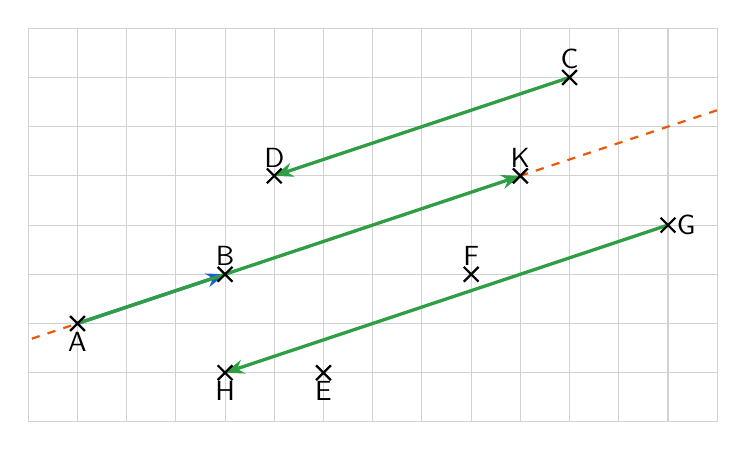
\begin{tikzpicture}[x=0.625cm,y=0.625cm]
\draw[gray!35,thin,step=0.625cm] (0,0) grid (14,8);
\begin{scope}\clip (0,0) rectangle (14,8);
\draw[ref] (-119,-38) -- (121,42);
\end{scope}
\draw[vec,vbleu] (1,2) -- (4,3);
\draw[vec,vert] (11,7) -- (5,5);
\draw[vec,vert] (13,4) -- (4,1);
\draw[vec,vert] (1,2) -- (10,5);
\node[ptcross] at (1,2) {}; \node[anchor=north,inner sep=3pt] at (1,2) {A};
\node[ptcross] at (4,3) {}; \node[anchor=south,inner sep=3pt] at (4,3) {B};
\node[ptcross] at (11,7) {}; \node[anchor=south,inner sep=3pt] at (11,7) {C};
\node[ptcross] at (5,5) {}; \node[anchor=south,inner sep=3pt] at (5,5) {D};
\node[ptcross] at (6,1) {}; \node[anchor=north,inner sep=3pt] at (6,1) {E};
\node[ptcross] at (9,3) {}; \node[anchor=south,inner sep=3pt] at (9,3) {F};
\node[ptcross] at (13,4) {}; \node[anchor=west,inner sep=3pt] at (13,4) {G};
\node[ptcross] at (4,1) {}; \node[anchor=north,inner sep=3pt] at (4,1) {H};
\node[ptcross] at (10,5) {}; \node[anchor=south,inner sep=3pt] at (10,5) {K};
\end{tikzpicture}\end{minipage}\hspace{0.5cm}\begin{minipage}[c]{7.1cm}{\color{vert}\Large Explication}\par\vspace{4pt}{\color{vert}$\V{CD}=-2\,\V{AB}$} : même direction, sens opposé ; la norme de $\V{CD}$ est deux fois plus grande que celle de $\V{AB}$.\par {\color{vert}$\V{GH}=-3\,\V{AB}$} : même direction, sens opposé ; la norme de $\V{GH}$ est trois fois plus grande que celle de $\V{AB}$.\par {\color{vert}$\V{AK}=3\,\V{AB}$} : même direction, même sens ; la norme de $\V{AK}$ est trois fois plus grande que celle de $\V{AB}$.\par {\color{gris}Avec les carreaux :} $\V{AB}$ : 3 vers la droite, 1 vers le haut ; $\V{CD}$ : 6 vers la gauche, 2 vers le bas ; $\V{GH}$ : 9 vers la gauche, 3 vers le bas ; $\V{AK}$ : 9 vers la droite, 3 vers le haut.\end{minipage}\end{minipage}
\end{document}
